% !TEX program = XeLaTeX
% !TEX encoding = UTF-8 Unicode

\documentclass[10pt,xcolor=svgnames]{beamer}

\usepackage[spanish]{babel}
\usepackage{fontawesome}

\usepackage{tikz,pgf}%,pgfarrows,pgfnodes,pgfautomata,pgfheaps}

\usepackage{booktabs}
\usepackage{multicol}
\usepackage{colortbl}
\usepackage{graphicx}
\graphicspath{{img/}}
\usepackage{blindtext}
\usepackage{keystroke}
%% Cajas
\usepackage[listings]{tcolorbox}

% Beamer configuration
\usetheme[sectionpage=progressbar,numbering=none,titleformat frame=smallcaps]{metropolis}
\setbeamertemplate{navigation symbols}{}

\usepackage{fontspec}
\setromanfont{TeX Gyre Pagella}

\definecolor{dblue}{rgb}{0.23,0.4,0.7}
\definecolor{azulon}{rgb}{0,0,0.44}
\definecolor{naranjon}{rgb}{.84,.418,0}
\definecolor{rojoclaro}{rgb}{.6,.2,0}
\definecolor{verdepaquete}{rgb}{.0,.4,.2}

\definecolor{codegreen}{rgb}{0,0.6,0}
\definecolor{codegray}{rgb}{0.5,0.5,0.5}
\definecolor{codepurple}{rgb}{0.58,0,0.82}
\definecolor{backcolour}{rgb}{0.95,0.95,0.92}

\usepackage{listings}
\lstset{
  language=[latex]tex,
  backgroundcolor=\color{backcolour},   
  commentstyle=\color{codegreen},
  keywordstyle=\color{magenta},
  numberstyle=\tiny\color{codegray},
  stringstyle=\color{codepurple},
  basicstyle=\ttfamily,%\footnotesize,
  breakatwhitespace=false,         
  breaklines=true,  
  firstnumber=1,
  %    captionpos=b,                    
  keepspaces=true,                 
  numbers=left,                    
  numbersep=5pt,                  
  showspaces=false,                
  showstringspaces=false,
  showtabs=false,                  
tabsize=2}

% minimizar fragmentado de listados
\lstnewenvironment{listing}[1][]
{\lstset{#1}\pagebreak[0]}{\pagebreak[0]}

\lstdefinestyle{consola}
{basicstyle=\scriptsize\bf\ttfamily}

\hypersetup{pdftitle={Introducción al lenguaje LaTeX para edición de textos académicos},
  pdfsubject={Curso de LaTeX}
  pdfauthor={Orientamat modificado por Francisco Torralbo}
  pdfkeywords={LaTeX, Orientamat},
  pdfpagemode={FullScreen},
  colorlinks,
  linkcolor=Orange,
}

\title{Introducción al lenguaje \LaTeX\ para edición de textos académicos}

\subtitle{Sesión 1: Instalación, personalización y primeros pasos}

\author{Orientamat (2017), modificado por Francisco Torralbo (2021)}

\institute{Universidad de Granada}

\date[2021]{26 de febrero de 2021}

\titlegraphic{
  
\includegraphics[width=.35\linewidth]{logo-ugr.pdf}\hfill
  
\includegraphics[width=.15\linewidth]{logo-yosigopublicando.jpg}
}

\begin{document}


\maketitle

\begin{frame}
  \frametitle{Estructura del Curso}
  \setbeamertemplate{section in toc}[sections numbered]
  \tableofcontents[hideallsubsections]
\end{frame}

\section{Preparación del material}

\begin{frame}{Descarga del contenido del curso}

  \url{github.com/latex-mat-ugr/curso-virtual-2021}

  \begin{center}
  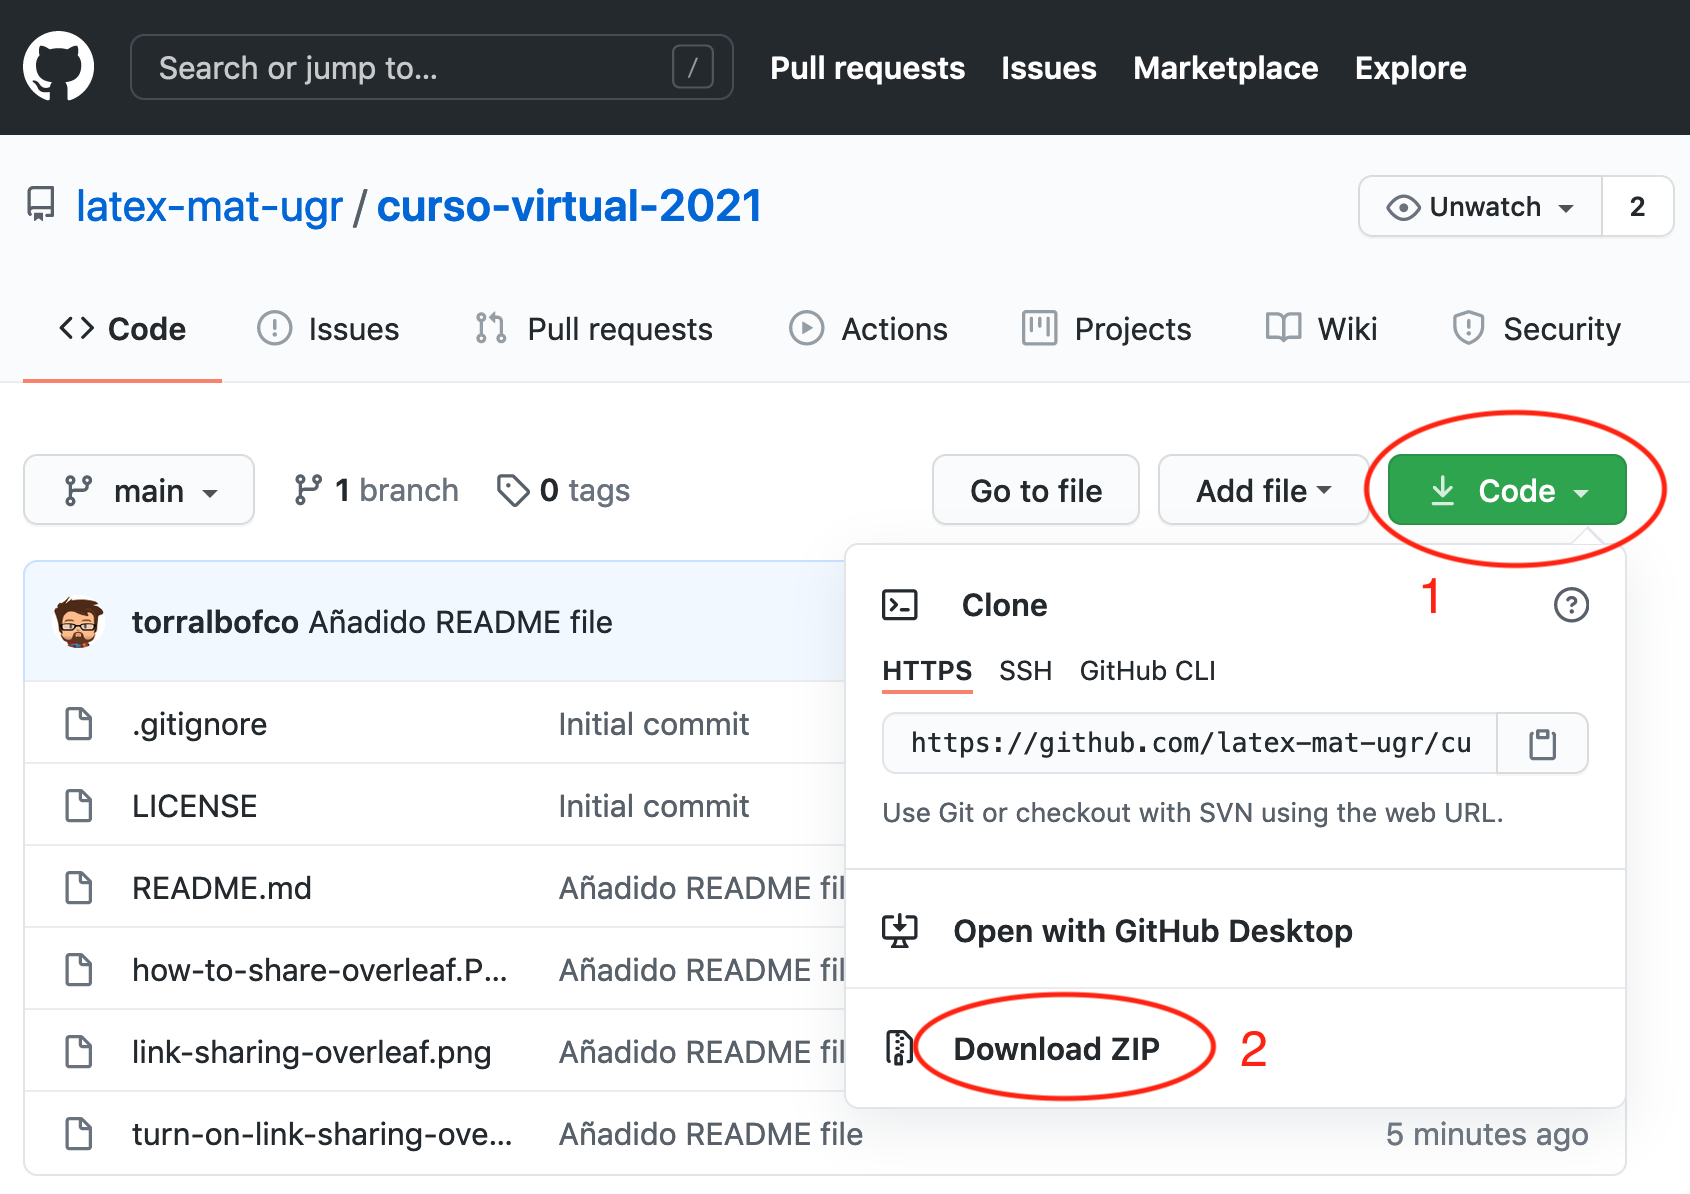
\includegraphics[width=0.6\linewidth]{download-repositorio-github.png} 
  \end{center}

  O usar \href{https://github.com/latex-mat-ugr/curso-virtual-2021/archive/main.zip}{este enlace}.

  \textbf{Importante}: Si vamos a usar el material en nuestro ordenador es imprescindible descomprimir el archivo en una carpeta.
\end{frame}

\begin{frame}{Subir el contenido a Overleaf}

  \begin{minipage}{0.25\linewidth}
    \small
    Crear un nuevo proyecto
  \end{minipage}
  \begin{minipage}{0.7\linewidth}
    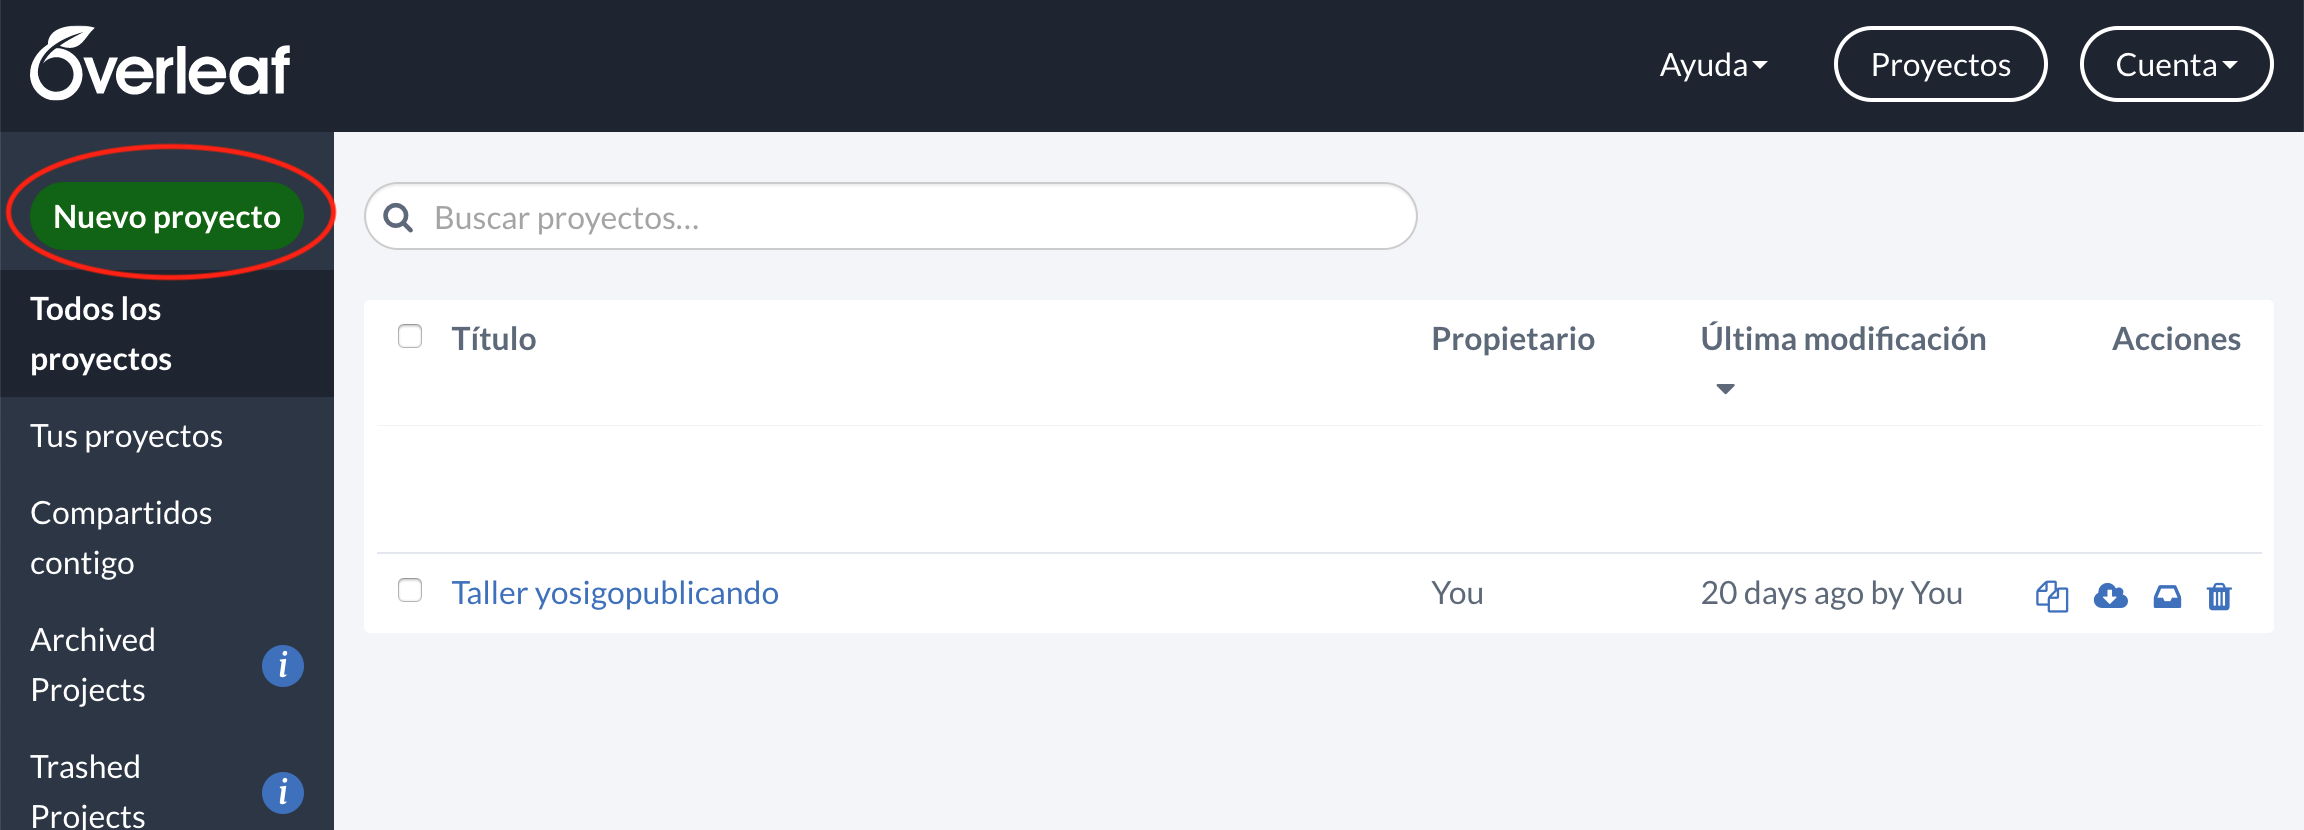
\includegraphics[width=\linewidth]{overleaf-crear-proyecto.png}
  \end{minipage}

  \begin{minipage}{0.25\linewidth}
    \small
    Subir un proyecto
  \end{minipage}
  \begin{minipage}{0.7\linewidth}
    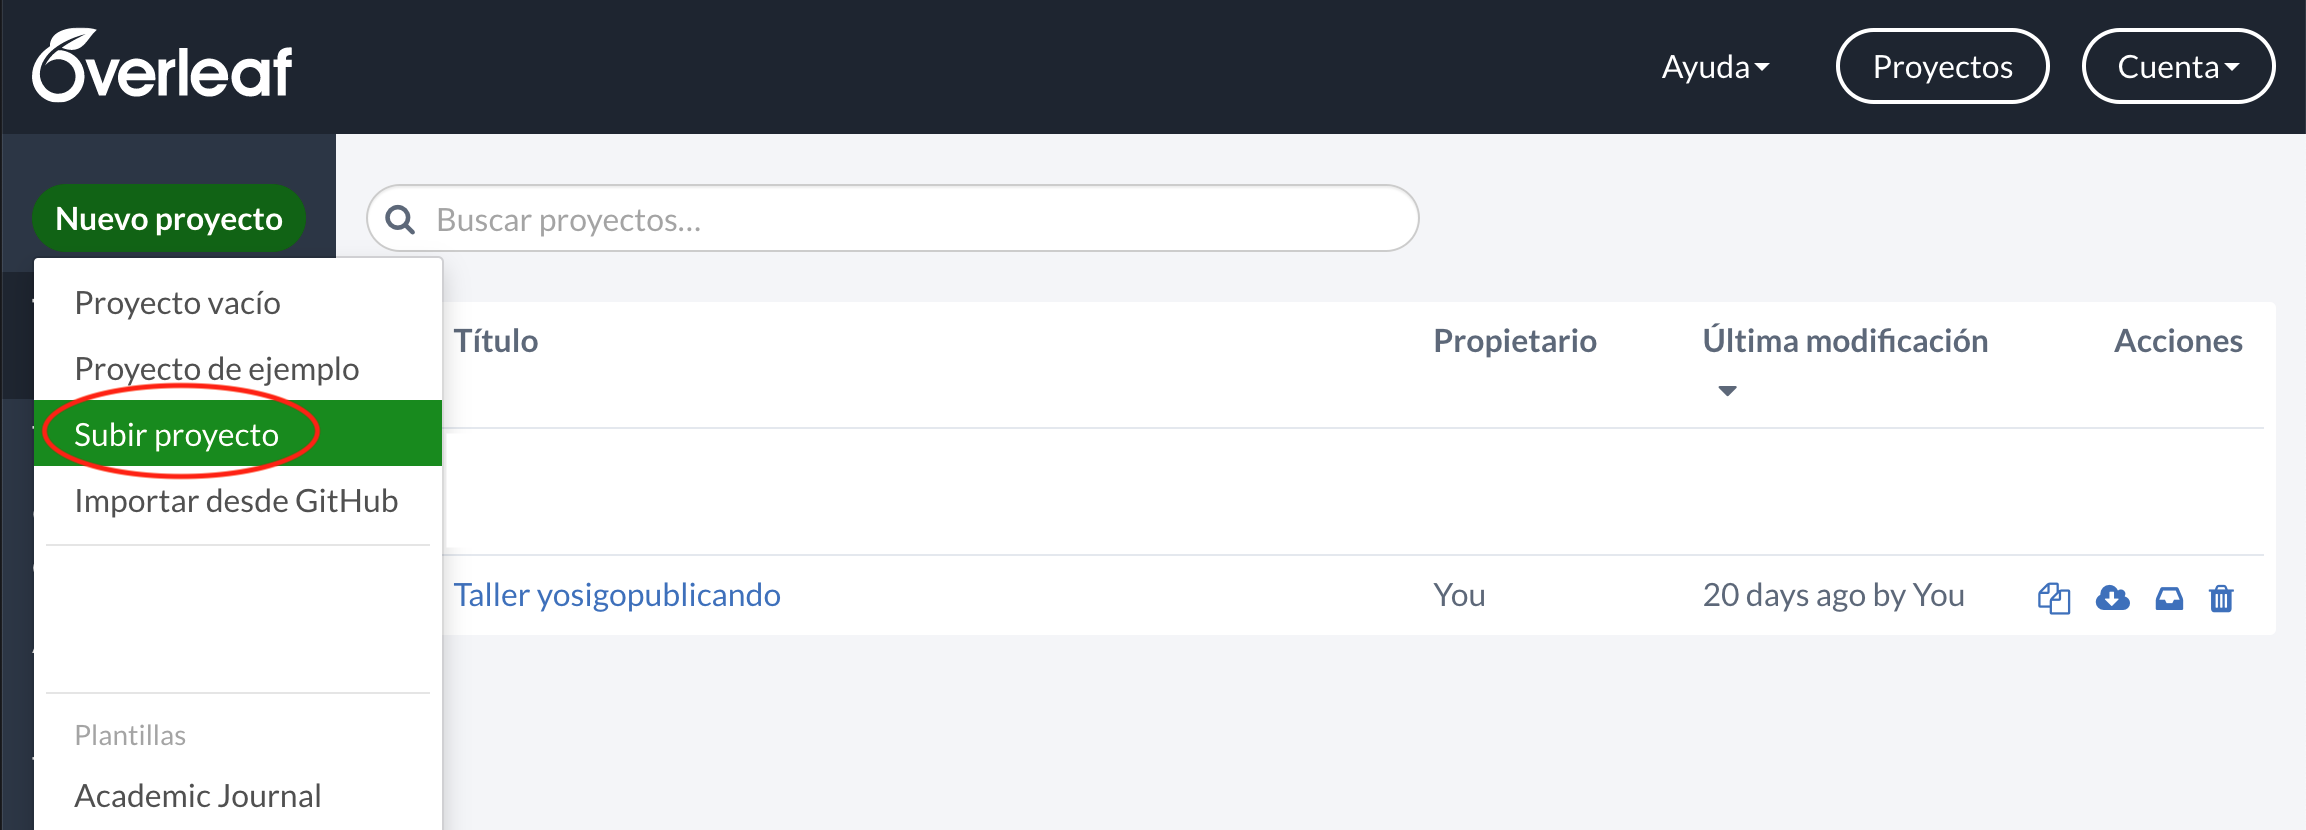
\includegraphics[width=\linewidth]{overleaf-subir-proyecto.png}
  \end{minipage}

  \begin{minipage}{0.25\linewidth}
    \small
    Arrastrar el archivo \texttt{zip} descargado
  \end{minipage}
  \begin{minipage}{0.7\linewidth}
    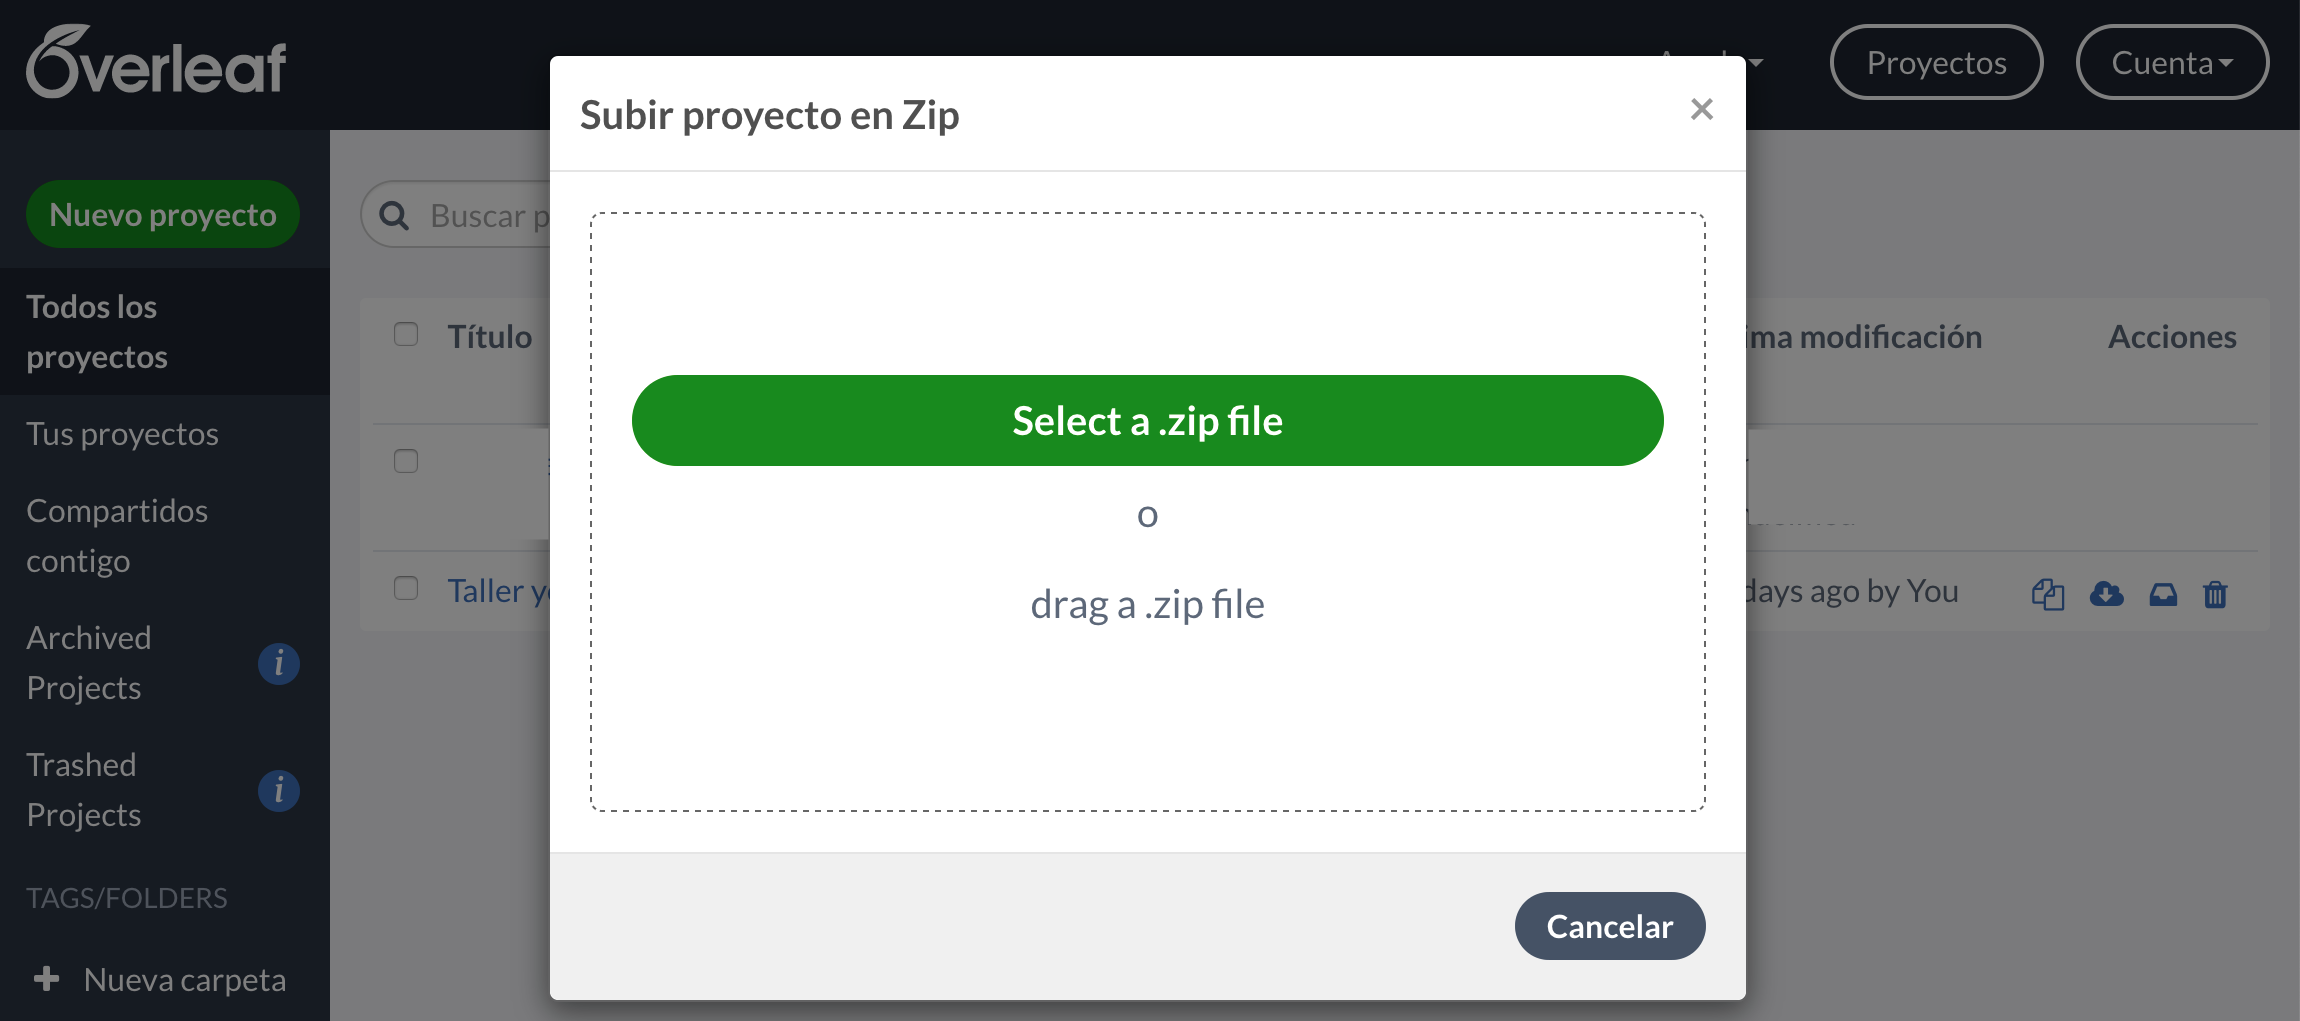
\includegraphics[width=\linewidth]{overleaf-arrastrar-zip.png}
  \end{minipage}

\end{frame}



\section{¿Qué es \LaTeX?}

\subsection{¿Qué es \LaTeX?}

\begin{frame}
  \frametitle{¿Qué es?}
  \begin{block}{¿Qué es \TeX?}
    \begin{itemize}
      \item \TeX{} es un programa destinado a la composición de documentos que contienen texto y fórmulas matemáticas con calidad de imprenta creado por Donald Knuth en 1978
      \item NO es un editor de texto sino un procesador de macros y lenguaje de programación
    \end{itemize}
  \end{block}
  \begin{block}{¿Y \LaTeX?}
    \begin{itemize}
      \item \LaTeX{} es un conjunto de macros para \TeX{}  debido originalmente a Leslie Lamport para facilitar el uso de \TeX.
      \item La Sociedad Matemática Americana añade sus estándares a \LaTeX{}: nace AMS-\LaTeX
    \end{itemize}
  \end{block}

  Usaremos el término \alert{\LaTeX{}} para referirnos a \TeX{} + \LaTeX{} + mejoras sucesivas
\end{frame}




\begin{frame}
  \frametitle{Características de \LaTeX}
  \begin{description}[Transportabiilidad]
    \addtolength\itemsep{\fill}
  \item[Transportable] los ficheros \texttt{.tex} sólo contienen texto y son de pequeño tamaño 
  \item[Estructurado] \LaTeX{} se ocupa del formato del documento. El usuario no tiene que preocuparse de hacer saltos de página, justificaciones, sangrías, referencias, etc.
  \item[Versátil] se puede hacer casi cualquier cosa (\href{https://www.tug.org/texshowcase/}{The \TeX\ showcase})
  \item[Flexible] permite al usuario crear nuevos comandos y entornos 
  \item[Actualizado] \LaTeX{} es mejorado constantemente de forma altruista.
\end{description}
\end{frame}


\begin{frame}[t,fragile]
  \frametitle{¿Cómo funciona?}
  \begin{block}{}
    \begin{itemize}
      \setlength{\itemsep}{0.5\baselineskip}
    \item Escribimos un fichero de texto con el contenido y órdenes
    \item \LaTeX{} lo procesa y da como resultado un fichero (PDF) formateado
  \end{itemize}
\end{block}

\begin{exampleblock}{Ejemplo}
  \begin{lstlisting}{language=tex}
\documentclass{article}
\begin{document}
    Consideremos una función \emph{continua} $f(x) = \cos(x)$. Su integral es...
\end{document}
  \end{lstlisting}

  Consideremos la función \emph{continua} $f(x)=\cos(x)$. Su integral es...
\end{exampleblock}
\end{frame}



\begin{frame}[t]
  \frametitle{Ventajas e inconvenientes}
  \vspace{-2em}
  \begin{columns}
    \begin{column}[t]{0.5\textwidth}
      \begin{block}{Ventajas}
        \begin{itemize}
          \item Composición de fórmulas
          \item Calidad de imprenta
          \item Facilidad para gestionar bibliografías, 
            notas, referencias, etc.
          \item Muchos paquetes adicionales
          \item Independiente de la plataforma: Unix, Windows, OSX,...
          \item Software libre
          \item Salida PDF, Postscript,...
          \item Separación de contenido y forma
        \end{itemize}
      \end{block}
    \end{column}
    \begin{column}[t]{0.5\textwidth}
      \begin{block}{Inconvenientes}
        \begin{itemize}
          \item Curva de aprendizaje lenta.
          \item El diseño de un documento es difícil 
            si los predefinidos no se ajustan a lo que necesitamos.
          \item Detección y manejo de errores.
        \end{itemize}
      \end{block}
    \end{column}
  \end{columns}
\end{frame}

\begin{frame}
  \frametitle{Distribuciones}
  \begin{itemize}
    \item \LaTeX{} está disponible en la mayoría de las plataformas usuales

    \item La \emph{distribuciones} más populares son
    \medskip

    \begin{itemize}
      \item \href{https://tug.org/texlive/}{\TeX Live} (\faApple, \faLinux, \faWindows)
      \item \href{https://miktex.org/}{MiK\TeX{}} (\faWindows)
      \item \href{https://www.tug.org/mactex/}{Mac\TeX{}} (\faApple)
    \end{itemize}

  \item Todas las distribuciones están basadas en el material disponible en \href{https://www.ctan.org/}{CTAN}: \emph{The comprehensive \TeX\ Archive Network}.	
\end{itemize}
\end{frame}


\begin{frame}
  \frametitle{Instalación}

  Es importante que tengamos instalado algún visor de archivos PDF.

  \begin{block}{En Windows \faWindows}
    \begin{itemize}
      %\setlength\itemsep{0.2\baselineskip}
      \item Vamos a instalar la distribución MiK\TeX
      \item Usaremos una variante de esta, \alert{Pro\TeX{t}}, que tiene incluidas algunos programas adicionales como TeXstudio o Ghostscript. 

        \centerline{\small \url{https://tug.org/protext/}}

    \end{itemize}
  \end{block}


  \begin{block}{En macOS \faApple}
    \begin{itemize}
      \item Usar \alert{Mac\TeX{}}  \quad {\small \url{https://tug.org/mactex/}}
    \end{itemize}
  \end{block}

  \begin{block}{En Linux \faLinux}
    \begin{itemize}
      \item Está disponible en los repositorios de las distribuciones
    \end{itemize}
  \end{block}
\end{frame}


\begin{frame}
  \frametitle{Editores}

  El programa (editor) que usemos para escribir un documento es independiente de \LaTeX{} aunque existen algunos editores mejor adaptados a su uso que incluyen atajos para algunas acciones usuales.
  \medskip

  Existen multitud de editores. Algunos son multiplataforma como el \href{https://www.texstudio.org/}{TeXstudio}, \href{https://www.xm1math.net/texmaker/}{TeXMaker} o \href{https://www.tug.org/texworks/}{TeXWorks} mientras que otros son específicos de cada sistema operativo, por ejemplo,
  \begin{description}
    \item[\faWindows] Texniccenter, Led,...
    \item[\faApple]  TeXShop,  scite,...
    \item[\faLinux] Kile, emacs, vim,...
  \end{description}
\end{frame}

\begin{frame}[fragile]
  \frametitle{Ayuda}
  \begin{block}{}
    \begin{itemize}
      % \addtolength{\itemsep}{0.5\baselineskip}
    \item Ayuda incluida en la instalación

    \item Manual básico: \href{https://osl.ugr.es/CTAN/info/lshort/spanish/lshort-a4.pdf}{La introducción no-tan-corta a \LaTeX 2$\varepsilon$} (la \href{https://tobi.oetiker.ch/lshort/lshort.pdf}{versión inglesa} suele estar más actualizada).

    \item \href{http://ctan.org}{CTAN}: documentación de todos los paquetes

    \item \href{https://www.tug.org/FontCatalogue/}{The TeX Font Catalogue}: documentación sobre las fuentes tipográficas incluidas en la instalación de \TeX.

    \item Listas de correo de Cervan\TeX\ \url{http://www.rediris.es/list/info/es-tex.html} 
    \item Foros, blogs, grupos de noticias, etc.
      \begin{itemize}
        \item \url{http://tex.stackexchange.com}
        \item \url{http://latex.org/forum/}
      \end{itemize}

    \item El repositorio público de \href{https://github.com/latex-mat-ugr}{\LaTeX\ para matemáticas para la Universidad de Granada}
  \end{itemize}
\end{block}
\end{frame}

\begin{frame}
  \frametitle{¿Para que sirve?}
  \begin{block}{Algunos usos}
    \begin{itemize}
      \addtolength{\itemsep}{0.5\baselineskip}
    \item Artículos,
    \item exámenes, ejercicios,
    \item cartas, informes,
    \item libros, apuntes, 
    \item \href{https://www.overleaf.com/latex/templates/tagged/poster}{posters}, \href{http://tug.ctan.org/macros/latex/contrib/beamer/doc/beameruserguide.pdf}{presentaciones}, \href{https://www.ctan.org/pkg/musixtex}{partituras}, etc.
  \end{itemize}
\end{block}
\end{frame}



\section{Creación de un documento \LaTeX}


\begin{frame}
  \frametitle{Ficheros \LaTeX}

  \begin{description}[.bib, .bbl, .blg, .bst]
    \item[.tex] Documento fuente: fichero de \emph{texto llano} que contiene tanto el contenido del documento como las instrucciones para estructurar dicho contenido. Se puede crear con cualquier editor de textos.
  \end{description}

  \bigskip

  Dicho documento se procesa (\emph{compila}) para obtener (generalmente) un \texttt{pdf}. Además se suelen generar varios archivos auxiliares:

  \medskip

  \begin{description}[.bib, .bbl, .blg, .bst]
    \addtolength\itemsep{0.5\baselineskip}
  \item[.aux] Contiene la información sobre las referencias, la bibliografía, el índice, etc.

  \item[.log] Mensajes del compilador.

  \item[.toc, .lof, .lot] Información relativa a índices, lista de figuras y lista de tablas.

  \item[.bib, .bbl, .blg, .bst] Ficheros relacionados con la bibliografía.

\end{description}

Dichos ficheros pueden borrarse al finalizar el documento.

\end{frame}





\subsection{Estructura de un documento \texttt{.tex}}

\begin{frame}[fragile]
  \frametitle{Partes de un documento \texttt{.tex}}

  Cualquier  documento \texttt{.tex} tiene dos partes: el \emph{encabezamiento} (o \emph{preámbulo}) y el \emph{cuerpo}

  \begin{block}{Encabezamiento o preámbulo}
    \begin{itemize}
      \addtolength\itemsep{0.5\baselineskip}
    \item Contiene la información sobre los aspectos globales del
      documento: tipo de documento, tipo de letra, márgenes, 
      espacio entre líneas, etc. y los paquetes adicionales.



    \item Comienza con la declaración del tipo de documento:

      \lstinline!\documentclass[opciones]{tipo de documento}!


  \end{itemize}
\end{block}

\begin{block}{Cuerpo}
  \begin{itemize}
    \addtolength\itemsep{0.5\baselineskip}
  \item Contiene el texto y los comandos
    para darle el formato deseado

  \item Se encuentra encerrado por el \emph{entorno}\\
    \lstinline!\begin{document} ... \end{document}! 
\end{itemize}
\end{block}
\end{frame}

\subsection{Escritura en el documento fuente}
\begin{frame}[fragile]
  \frametitle{Escritura en el documento fuente}
  Hay que tener en cuenta que el aspecto final del documento \emph{no} se asemejará en absoluto al documento \texttt{.tex}

  \begin{block}{}
    En el documento fuente escribimos como si tuviésemos una línea infinita, que luego \LaTeX{} interpretará.
    \begin{itemize}
      \item \LaTeX{} finaliza las líneas donde considera más oportuno, justifica el texto por la derecha (realizando segmentación silábica) y realiza sangría por la izquierda al comienzo de cada párrafo
      \item Para cambiar de párrafo debemos \emph{dejar una línea en blanco} o escribir \lstinline!\par!
    \end{itemize}
  \end{block}

\end{frame}

\begin{frame}[t,fragile]
  \frametitle{Primer ejemplo}
  \begin{exampleblock}{Nuestro primer texto en \LaTeX}
    \begin{lstlisting}{language=tex}
\documentclass[a4paper]{article}

\begin{document}
Pasos para instalar Latex en nuestro ordenador. 
Mejor dicho, Latex se escribe \LaTeX.

Los espacios en blanco no cuentan y si queremos 
empezar un párrafo nuevo sólo tenemos que dejar 
una línea en blanco. También podemos escribir 
fórmulas
\[
f(x)=\cos(x)+\frac{1}{x}
\]
\end{document}
    \end{lstlisting}
  \end{exampleblock}
\end{frame}


\begin{frame}[t,fragile]
  \frametitle{Primer ejemplo - Cabecera}
  \begin{lstlisting}
\documentclass[11pt]{article} % Tipo de documento

% Preámbulo ---------------------------------------
\usepackage[utf8]{inputenc} % Para escribir acentos
\usepackage{amsmath,amssymb,amsfonts,amsthm} 
  % matemáticas de la AMS
\usepackage[spanish]{babel} % selección del idioma
\usepackage[margin=3cm, a4paper]{geometry} % tamaño
% Fin del preámbulo -------------------------------

\begin{document}
  Texto del documento
\end{document}
  \end{lstlisting}

  \texttt{\%} se utiliza para añadir comentarios

\end{frame}

\begin{frame}[standout]
  \frametitle{Compilación}

  \begin{itemize}
    \setlength{\itemsep}{\baselineskip}
  \item ¿Cómo se compila?
  \item ¿Errores?
\end{itemize}

\end{frame}



\subsection{Errores en la compilación}
\begin{frame}{Gestión de errores en la compilación}
  Si \LaTeX{} encuentra errores en la compilación, para y se ``queja''. 

  \medskip

  \begin{block}{Posibles respuestas}
    \begin{description}
      \addtolength\itemsep{0.5\baselineskip}
    \item[\keystroke{Enter}] le estamos diciendo olvida el error y haz lo que puedas. Puede ser necesario repetir el proceso varias veces
    \item[\keystroke{x}+\keystroke{Enter}] \LaTeX{} para la compilación
    \item[\keystroke{r}+\keystroke{Enter}] \LaTeX{} seguirá aunque encuentre errores
    \item[\keystroke{e}+\keystroke{Enter}] \LaTeX{} para la compilación y nos manda al archivo fuente a la primera línea de código en la que encontró un error
  \end{description}
\end{block}

Es fácil que la línea que señala \LaTeX{} no sea donde este se encuentre.

\end{frame}




\section{Primeros pasos}

\subsection{Comandos y entornos}

\begin{frame}[fragile]
  \frametitle{Comandos}
  \begin{alertblock}{Comandos}
    \begin{itemize}
      \setlength{\itemsep}{0.5\baselineskip}
    \item Sirven para que \LaTeX{} realice una acción sencilla: cambiar de párrafo, escribir un símbolo, dejar un espacio\dots
    \item Comienzan con \texttt{\textbackslash} y se escriben sólo con letras (distingue mayúsculas y minúsculas)
    \item Pueden ser redefinidos y se pueden crear nuevos comandos
    \item La sintaxis habitual es:

      {\small \lstinline!\nombrecomando[opciones]{argumentos obligatorios}!}

    \item \LaTeX{} ignora los espacios después de un comando
  \end{itemize}
\end{alertblock}
\end{frame}

\begin{frame}[fragile]
  \frametitle{Comandos}

  \begin{exampleblock}{Ejemplos}
    \begin{itemize}
      \item \lstinline!\xi! escribe la letra griega xi: $\xi$.
      \item \lstinline!\emph{texto}! enfatiza un texto (normalmente en cursiva).
      \item \lstinline!\usepackage[spanish]{babel}! le dice a \LaTeX{} que cargue el paquete babel con la opción español.
    \end{itemize}
  \end{exampleblock}


  \begin{lstlisting}{language=tex}
Un documento contiene \textbf{texto} en negrita, 
letras griegas $\xi$. \emph{Texto resaltado}.
  \end{lstlisting}

\end{frame}

\begin{frame}
  \frametitle{Entornos}
  \begin{alertblock}{Entornos}
    \begin{itemize}
      \item Son órdenes que sirven para que \LaTeX{} realice una acción compleja: crear una matriz, crear un página dentro de otra, escribir en varias columnas\dots
      \item Es necesario abrir el entorno y cerrarlo, la sintaxis es: \par \texttt{\textbackslash begin\{entorno\} \... \textbackslash end\{entorno\}}
      \item Los entornos también se pueden redefinir y se pueden crear otros nuevos
    \end{itemize}
  \end{alertblock}

  \begin{exampleblock}{Ejemplos}
    \begin{itemize}
      \item Entornos para escribir listas: \texttt{itemize}, \texttt{enumerate}.
      \item Entornos para escribir tablas: \texttt{table}, \texttt{array}, matrix
      \item Entornos para situar el texto: \texttt{center}, \texttt{flushleft}, \texttt{flushright}.
    \end{itemize}
  \end{exampleblock}

  %Suele ser una buena estrategia cerrar los entornos justo después de abrirlos y luego continuar con el contenido del entorno.
\end{frame}

\begin{frame}[t,fragile]
  \frametitle{Paquetes}

  \LaTeX\ es \textbf{modular}: su comportamiento y características pueden ser modificados o ampliados a través de paquetes.

  Un \textbf{paquete} es un \emph{conjunto de instrucciones} de \LaTeX\ diseñado para resolver un problema concreto del documento. 

  Para cargar un paquete escribiremos el siguiente \emph{comando} en el \emph{preámbulo} del documento:

\begin{lstlisting}{language=tex}
\usepackage[opciones]{paquete}
\end{lstlisting}

Existen multitud de paquetes que cubren la mayoría de las necesidades del usuario: aspecto del documento, manejo de índice, glosario, referencias, idioma, hipervínculos,...Buscar en \href{https://www.ctan.org}{CTAN}.

  Si tienes algún problema o quieres hacer algo específico en \LaTeX\ seguramente exista un paquete que lo resuelva.


\end{frame}


\subsection{Grupos}
\begin{frame}[fragile]
  \frametitle{Grupos}


  \begin{alertblock}{Grupo}
    Es una parte bien delimitada del documento, con un inicio y un fin y que abarca todo lo que hay comprendido entre ambos
    \medskip
    \begin{itemize}
      \item Para abrir un grupo utilizamos \texttt{\color{magenta}\{} y para cerrarlo \texttt{\color{magenta}\}}
        \medskip
      \item Los grupos se pueden anidar unos dentro de otros
    \end{itemize}
  \end{alertblock}
\end{frame}


\begin{frame}[fragile]
  \frametitle{Grupos}
  \begin{exampleblock}{Ejemplo}

\begin{lstlisting}{language=tex}
\textsc{Queremos escribir una frase en letras 
mayúsculas pequeñas {\color{blue} y una parte 
dentro de ella en \textbf{azul}} y a su vez 
otras partes  en \textbf{negrita} y otra más 
{\Large grande}}
\end{lstlisting}

    \medskip

\textsc{Queremos escribir una frase en letras 
mayúsculas pequeñas {\color{blue} y una parte 
dentro de ella en \textbf{azul}} y a su vez 
otras partes  en \textbf{negrita} y otra más 
{\Large grande}}

    % \includegraphics[width=\linewidth]{text.pdf}
  \end{exampleblock}
\end{frame}


\subsection{Estructura del documento}

\begin{frame}[fragile]{Estructura del documento}

Todo documento tiene una estructura interna. Dependiendo del tipo de documento (artículo, informe, libro,\ldots) esa estructura será diferente. \LaTeX\ proporciona los siguientes comandos para definir la estructura del documento:

\begin{itemize}
  \item \lstinline!\part! Para dividir el documento en partes (clases \texttt{book} y \texttt{report})
  \item \lstinline!\chapter! Para los capítulos (clases \texttt{book} y \texttt{report})
  \item \lstinline!\section! Para las secciones
  \item \lstinline!\subsection! Para las subsecciones
  \item \lstinline!\subsubsection! Para las secciones de tercer nivel
\end{itemize}

Una vez estructurado nuestro documento usando los anterior comandos podemos mostrar la tabla de contenido. Para ello bastará con incluir el siguiente comando (generalmente después del título del documento) para \emph{generar} dicha tabla:

\begin{lstlisting}{language=tex}
\tableofcontents
\end{lstlisting}


\end{frame}


\begin{frame}[fragile]{Título y autor de un documento}

En las clases estándar de \LaTeX\ (\texttt{book}, \texttt{report}, \texttt{article}) existen comandos para definir el título y autor de un documento y mostrarlos con cierto formado predefinido:

\begin{lstlisting}{language=tex}
\documentclass{article} % book, report
% Preámbulo
\begin{document}

  \title{Documento de ejemplo de \LaTeX}
  \author{Leonar Euler \and Bernard Riemann}
  \date{} % Dejar vacío si no queremos que se imprima la fecha

  \maketitle
  \tableofcontents

\end{document}
\end{lstlisting}

\end{frame}


\subsection{Líneas, párrafos y páginas}


\begin{frame}[fragile]
  \frametitle{Líneas y párrafos}
La unida básica de estructura es el párrafo que se delimita por al menos una línea vacía antes y después de él.
  \begin{alertblock}{Espacios y párrafos}
    \begin{itemize}
      \addtolength\itemsep{0.5\baselineskip}
    \item Uno o más espacios son tratados como un espacio.
    \item También se trata como un espacio el salto de línea.

    \item Varias líneas en blanco separan los párrafos.
    \item El comando \lstinline!\par! tiene el mismo efecto.

    \item \lstinline!\newline! inicia una nueva línea sin completar la línea en curso
    \item \lstinline!\linebreak[opcion]! inicia una nueva línea justificando la línea en curso
  \end{itemize}
\end{alertblock}

\end{frame}


\begin{frame}[t,fragile]
  \frametitle{Alineación de párrafos}



  \begin{block}{Alinear}
    Se pueden alinear a izquierda o derecha párrafos usando
    \begin{lstlisting}{language=tex}
\begin{flushleft}
Alineado a la izquierda\ldots
\end{flushleft}
\begin{flushright}
\ldots alineado a la derecha.
\end{flushright}
    \end{lstlisting}
  \end{block}

  \begin{block}{Centrar párrafos}
    Se pueden centrar párrafos con 
    \begin{lstlisting}{language=tex}
\begin{center}
Esto es un texto centrado
\end{center}
    \end{lstlisting}
  \end{block}

\end{frame}


\begin{frame}[fragile]
  \frametitle{Párrafos}

  \begin{block}{}
    \begin{itemize}
      \addtolength\itemsep{0.5\baselineskip}
    \item Hay entornos (quote, quotation, verse) para escribir algunos tipos de párrafos particulares

    \item Se puede cambiar el espacio entre líneas de varias formas. Se recomienda usar el paquete \texttt{setspace} %(aunque también se pueden cambiar el valor de linespread o baselinestrecth)
      \begin{lstlisting}
\usepackage{setspace}
\onehalfspacing % linea y media
\doublespacing % doble espacio
      \end{lstlisting}

    \item 
      \LaTeX{} realiza una sangría a la izquierda al comienzo de cada nuevo párrafo. Si se quiere evitar se utiliza el comando \lstinline!\noindent!
  \end{itemize}
\end{block}
\end{frame}



\begin{frame}[fragile]
  \frametitle{Espacios, párrafos y páginas}

  \begin{block}{Saltos de página}
    \begin{itemize}
      \addtolength\itemsep{0.5\baselineskip}
    \item \lstinline!\newpage! inicia una nueva página sin completar la página en curso
    \item \lstinline!\clearpage! produce un efecto similar al comando anterior ubicando los objetos ``flotantes'' (como tablas o gráficos) en una nueva página sin texto alguno
  \end{itemize}
\end{block}


\end{frame}



\subsection{Símbolos especiales}
\begin{frame}{Símbolos especiales}
  \begin{block}{Símbolos reservados}

    Algunos caracteres tienen una utilidad especial para \LaTeX{} y su uso está reservado. Todos se pueden escribir anteponiendo una barra invertida salvo la propia barra invertida (\textbackslash{}\textbackslash indica línea nueva)
    \begin{description}[\^{} y \_{}]
      \addtolength\itemsep{0.4\baselineskip}
    \item[\${}] Declarar el modo matemático {\color{rojoclaro}$\backslash$}{\color{blue}\$}
    \item[\{{} \}{}] Iniciar y finalizar grupos {\color{magenta}{\color{rojoclaro}$\backslash$}\{\qquad{\color{rojoclaro}$\backslash$}\}}
    \item[\#{}] Indicar el número de un argumento {\color{rojoclaro}$\backslash$}{\color{magenta}\#}
    \item[\%{}] Hacer que \LaTeX{} ignore una línea de código {\color{magenta}\lstinline!\\\%!}
    \item[\&{}] Separar elementos de una tabla o una fórmula {\color{magenta}\lstinline!\\&!}
    \item[\textbackslash{}] Inicio de cualquier comando {\color{blue}\$}{\color{rojoclaro}$\backslash$}backslash{\color{blue}\$}
    \item[\^{} y \_{}] Escribir super y subíndices {\color{rojoclaro}\lstinline!\\^!\qquad \lstinline!\\_!}
    \item[\~{}] ``Pegar'' palabras {\color{rojoclaro}\lstinline!\\~!}
  \end{description}
\end{block}
\end{frame}

\begin{frame}{Símbolos especiales}
  \begin{block}{Símbolos ortográficos}
    \begin{itemize}
      \addtolength\itemsep{0.5\baselineskip}
    \item Es mejor usar el paquete \emph{inputenc} con la codificación adecuada que escribir el comando necesario para cada símbolo.

    \item ¿Cómo se escriben las <<comillas>>, ``comillas''?

    \item ¿Y los puntos suspensivos\ldots?

    \item ¿Y los ordinales? 1\sptext{o} (¿o es 1º?) 
  \end{itemize}
\end{block}

\end{frame}




\begin{frame}[fragile]
  \frametitle{División de palabras}

  \begin{block}{}
    \begin{itemize}
      \addtolength\itemsep{0.5\baselineskip}
    \item \LaTeX{} se encarga de la división de palabras al final de línea cuando sea necesario.

    \item Se puede indicar como dividir una palabra concreta usando \textbackslash{}-

    \item El comando \lstinline!\hyphenation{pa-la-bra1, pa-la-bra2,...}! en la cabecera vale para todo el documento.

    \item El paquete \texttt{babel} hace, entre otras cosas, que \LaTeX{} use los patrones de guionado del lenguaje seleccionado.

  \end{itemize}
\end{block}

\end{frame}








\subsection{Tipos y colores}

% \begin{frame}{Tipos}
%   Las familias tipográficas 

%   Codificación (paquete \texttt{fontenc})

%   \begin{tikzpicture}[every node/.style={inner sep=0.25cm,font=\sffamily\bfseries}]
%     % Overlaying rectangles
%     \begin{scope}[fill=yellow!65!red,nearly transparent]
%         % Series
%         \fill (-4.25,-2) rectangle (4.25,2);
%         \draw [white, opaque, ultra thick] (0,-2) -- (0,2);
%         % Size
%         \fill (-1.5,-2) rectangle (1.5,2);
%         % Family
%         \fill (-4.5,-2.25) rectangle (4.5,2.75);
%         % Encoding
%         \fill (-4.75,-2.5) rectangle (4.75,3.5);
%     \end{scope}
%     % Text
%     \node {Tamaño};
%     \node at (-4,0)      [right]       {Grosor};
%     \node at (-4,-0.5)      [right]       {(\emph{series})};
%     \node at (4,0)       [left]        {Perfiles};
%     \node at (4,-0.5)       [left]        {(\emph{shape})};
%     \node at (-4.5,2.75) [below right] {Familia (\emph{family})};
%     \node at (-4.75,3.5) [below right] {Fuente};
% \end{tikzpicture}

% % https://tex.stackexchange.com/questions/7669/bfseries-is-to-textbf-as-what-is-to-textsf/7670#7670
% \end{frame}

\begin{frame}[fragile]{Comandos para cambiar el estilo tipográfico}
  \tiny
  \rmfamily

  \noindent
  \begin{tabular}{ll|llll|l}
    \toprule 
    \multicolumn{2}{c}{Familia} & \multicolumn{4}{c}{Estilo} & \multicolumn{1}{c}{Tamaño} \\ \cmidrule{3-6}
                               & & \multicolumn{2}{c}{Grosor (series)} & \multicolumn{2}{c}{Perfil (shape)} &
    \\\midrule
    \textrm{Serif} & \verb+\textrm+ & Normal & \verb+\textmd+ & Recto & \verb+\textup+ & {\tiny\verb+\tiny+} \\
                            & \verb+\rmfamily+ & & \verb+\mdseries+ & & \verb+\upshape+ & {\scriptsize\verb+\scriptsize+} \\
    \textsf{sans-serif} & \verb+\textsf+ & \textbf{Negrita} & \verb+\textbf+ & \textit{Cursiva} & \verb+\textit+ & {\footnotesize\verb+\footnotesize+} \\
                            & \verb+\sffamily+ & & \verb+\bfseries+ & & \verb+\itshape+ & {\small\verb+\small+} \\
    \texttt{Monoespaciada} & \verb+\texttt+ & & & \textsl{Inclinada} & \verb+\textsl+ & {\normalsize\verb+\normalsize+} \\
                            & \verb+\ttfamily+ & & & & \verb+\slshape+ & {\large\verb+\large+} \\
                            & & & & \textsc{Versalitas} & \verb+\textsc+ & {\Large\verb+\Large+} \\
                            & & & & & \verb+\scshape+ & {\LARGE\verb+\LARGE+} \\
                            & & & & & & {\huge\verb+\huge+} \\
                            & & & & & & {\Huge\verb+\Huge+} \\
    \bottomrule
  \end{tabular}

  \textit{\textbf{\textrm{\normalsize Texto compuesto en la fuente ``TeX Gyre Pagella'' en serif negrita cursiva a tamaño normal.}}}
\end{frame}

\begin{frame}[fragile]
  \frametitle{Ejemplos}
  \begin{block}{Familias de tipos de letra}
    %Hay tres tipos de letra:
    \begin{description}[\texttt{Máquina de escribir}]
      \item[Texto normal] \lstinline!\textrm{Texto}! \quad $\rightsquigarrow$ \textrm{Texto}
      \item[\textsf{Sanserif o sin adornos}] \lstinline!\textsf{Texto}! \quad $\rightsquigarrow$ \textsf{Texto}
      \item[\texttt{Máquina de escribir}] \lstinline!\texttt{Texto}! \quad $\rightsquigarrow$ \texttt{Texto}
    \end{description}
  \end{block}


  \bigskip

  \begin{block}{Perfiles}
    \begin{description}[\texttt{Máquina de escribir}]
      \item[Recto]  \lstinline!\textup{Texto}! \quad $\rightsquigarrow$ \textup{Hola}
      \item[Itálica] \lstinline!\textit{Texto}! \quad $\rightsquigarrow$ \textit{Hola}
      \item[Inclinado]  \lstinline!\textsl{Texto}! \quad $\rightsquigarrow$ \textsl{Hola}
      \item[Versalita]  \lstinline!\textsc{Texto}! \quad $\rightsquigarrow$ \textsc{Hola}
    \end{description}
  \end{block}

\end{frame}


\begin{frame}{Ejemplos}

  \begin{block}{Grosor}
    \begin{description}[\texttt{Máquina de}]
      \item[Normal]  \texttt{\textbackslash{}textmd\{Texto\}} \quad  $\rightsquigarrow$ \textmd{hola}  
      \item[Grueso]  \texttt{\textbackslash{}textbf\{Texto en negritas\}} \quad $\rightsquigarrow$ \textbf{hola}
    \end{description}
  \end{block}

  \bigskip

  \begin{block}{Otras formas de destacar texto}
    \begin{description}[\texttt{Máquina de}]
      \item[Resaltar] \texttt{\textbackslash emph\{Texto a resaltar\}} \quad $\rightsquigarrow$ \emph{hola}
      \item[Subrayar] \texttt{\textbackslash{}underline\{Texto subrayado\}} \quad $\rightsquigarrow$ \underline{hola}
    \end{description}
  \end{block}

\end{frame}



\begin{frame}[fragile]
  \frametitle{Tamaños}

  \begin{block}{Tamaño de letra}
    \begin{lstlisting}{language=tex}
{\tiny Hay} {\footnotesize unos} {\small pocos} 
{\normalsize tamaños} {\large de} {\Large letra} 
{\huge en} {\Huge \LaTeX} {\huge que} {\Large se} 
{\large ponen} {\normalsize con} {\small los}
{\footnotesize comandos} {\tiny siguientes}
    \end{lstlisting}
    \medskip

    {\tiny Hay} {\footnotesize unos} {\small pocos} 
    {\normalsize tamaños} {\large de} {\Large letra} 
    {\huge en} {\Huge \LaTeX} {\huge que} {\Large se} 
    {\large ponen} {\normalsize con} {\small los}
    {\footnotesize comandos:}

    \texttt{
      {\tiny$\backslash$tiny}
      {\scriptsize$\backslash$scriptsize}
      {\footnotesize$\backslash$footnotesize}
    {\small$\backslash$small}} \texttt{\normalsize$\backslash$normalsize}

    \texttt{{\large$\backslash$large}
      {\Large$\backslash$Large}
      {\LARGE$\backslash$LARGE}
      {\huge$\backslash$huge}
    {\Huge $\backslash$Huge}}
  \end{block}
\end{frame}





\subsection{Listas}

\begin{frame}[fragile,t]
  \frametitle{Listas}
  \framesubtitle{Listas numeradas}
  Existen tres entornos en \LaTeX{} para escribir listas: \alert<2->{enumerate}, itemize y description.

  \bigskip \bigskip

  \pause
  \textbf{Entorno enumerate}


  \begin{columns}
    \begin{column}[]{0.5\textwidth}
\begin{lstlisting}{language=tex}
\begin{enumerate}
   \item Primer ítem,
   \item segundo ítem, y
   \item tercer ítem.
\end{enumerate}
\end{lstlisting}
    \end{column}
    \begin{column}[]{0.5\textwidth}
      \begin{enumerate}
        \item Primer ítem,
        \item segundo ítem, y
        \item tercer ítem.
      \end{enumerate}
    \end{column}
  \end{columns}


\end{frame}

\begin{frame}[fragile,t]
  \frametitle{Listas}
  \framesubtitle{Listas con viñetas}
  Existen tres entornos en \LaTeX{} para escribir listas: enumerate, \alert<2->{itemize} y description.

  \bigskip \bigskip

  \pause

  \textbf{Entorno itemize}



  \begin{columns}
    \begin{column}[]{0.5\textwidth}
\begin{lstlisting}{language=tex}
\begin{itemize}
   \item Primer ítem,
   \item segundo ítem, y
   \item tercer ítem.
\end{itemize}
\end{lstlisting}
    \end{column}
    \begin{column}[]{0.5\textwidth}
      \begin{itemize}
        \item Primer ítem,
        \item segundo ítem, y
        \item tercer ítem.
      \end{itemize}	
    \end{column}
  \end{columns}


\end{frame}


\begin{frame}[fragile,t]
  \frametitle{Listas}
  \framesubtitle{Listas descriptivas}
  Existen tres entornos en \LaTeX{} para escribir listas: enumerate, itemize y
  \alert<2->{description}.

  \bigskip \bigskip

  \pause
  \textbf{Entorno description}


  \begin{columns}
    \begin{column}[]{0.48\textwidth}
\begin{lstlisting}{language=tex}
\begin{description}
   \item[Curso] Dirección o carrera.
   \item[Alumno] Discípulo, respecto de su maestro...
   \item[Maestro] Dicho de un irracional.
\end{description}
\end{lstlisting}
    \end{column}
    \begin{column}[]{0.48\textwidth}
      \begin{description}
        \item[Curso] Dirección o carrera.
        \item[Alumno] Discípulo, respecto de su maestro...
        \item[Maestro] Dicho de un irracional.
      \end{description}
    \end{column}
  \end{columns}


\end{frame}


\begin{frame}[fragile,t]
  \frametitle{Listas}

  Las listas se pueden anidar


  \bigskip \bigskip

  \begin{columns}
    \begin{column}[]{0.5\textwidth}
      \begin{lstlisting}{language=tex}
\begin{itemize}
  \item Varias cosas:
    \begin{enumerate}
       \item Una;
       \item otra;
       \item la última.
    \end{enumerate}
  \item segundo ítem y
  \item tercer ítem.
\end{itemize}
      \end{lstlisting}
    \end{column}
    \begin{column}[]{0.5\textwidth}
      \begin{itemize}
        \item Varias cosas:
          \begin{enumerate}
            \item Una;
            \item otra;
            \item la última.
          \end{enumerate}
        \item segundo ítem y
        \item tercer ítem.
      \end{itemize}
    \end{column}
  \end{columns}

\end{frame}


\begin{frame}[t]
  \frametitle{Listas}

  \begin{block}{¿Y después?}
    \begin{enumerate}
      \item El formato, la numeración, las vi\~{n}etas, el espaciado, sangrado, etc. se pueden modficar.
      \item Todas las listas que hemos visto son un caso particular del entorno ``list''. Se pueden definir listas personalizadas.
    \end{enumerate}
  \end{block}

  \bigskip \bigskip

  \begin{block}{Ejercicios}
    \begin{enumerate}
      \item Prueba a anidar listas de diferentes tipos
      \item ¿Qué ocurre si anidas m\'{a}s de cuatro?
    \end{enumerate}
  \end{block}
\end{frame}



\subsection{Matemáticas}

\begin{frame}[fragile]
  \frametitle{Matemáticas}
  Podemos escribir fórmula \alert{en línea}, $\sqrt{x+y}$ o en centradas en una línea separada
  \[
    \frac{\partial f}{\partial x} (x,y)= \sum_{n=1}^{\infty} \oint_{a}^{b} \frac{x}{1+x^2}\, \mathrm{d}x
  \]
  \begin{lstlisting}
Podemos escribir fórmula \alert{en línea}, 
$\sqrt{x+y}$ o en centradas en una línea separada
\[
f(x,y)= \sum_{n=1}^{\infty} \int_{a}^{b} 
\frac{x}{1+x^2}\, \mathrm{d}x
\]
  \end{lstlisting}

\end{frame}


\subsection{Bibliografía}

\begin{frame}[fragile]{Bibliografía de un documento}
\framesubtitle{Método director}

Todo el material utilizado para la elaboración de un trabajo ha de ser citado adecuadamente durante el texto. Al final de nuestro trabajo aparecerá una lista con las referencias que permiten localizar las fuentes usadas: La bibliografía.

\LaTeX\ proporciona el entorno \texttt{thebiliography} para listar la bibliografía de un documento

\begin{lstlisting}{language=tex}
\begin{thebibliography}{sangrado}

  \bibitem[Nombre1]{Etiqueta1} Datos bibliográficos
  \bibitem[Nombre2]{Etiqueta2} Datos bibliográficos

\end{thebibliography}
\end{lstlisting}

y el comando \lstinline!\cite! para hacer referencia a un elemento bibliográfico usando la \emph{etiqueta} indicada.

\end{frame}

\begin{frame}[fragile]{Bibliografía: Método directo. Ejemplo}
\framesubtitle{Ejemplo de bibliografía}

{\scriptsize
\begin{lstlisting}{language=tex}
\begin{thebibliography}{Eul85}

\bibitem[Eul]{EulerWiki} % Recurso online
{L}eonhard {E}uler.
\newblock \url{https://en.wikipedia.org/wiki/Leonhard_Euler}.
\newblock Recurso online. Accedido el 14 de marzo de 2019.

\bibitem[Eul84]{Euler1984} % Libro
Leonhard Euler.
\newblock {\em Elements of algebra}.
\newblock Springer-Verlag, New York, 1984.
\newblock Translated from the German by John Hewlett, Reprint of the 1840
  edition, With an introduction by C. Truesdell.

\bibitem[Eul85]{Euler1985} % Artículo
Leonhard Euler.
\newblock An essay on continued fractions.
\newblock {\em Math. Systems Theory}, 18(4):295--328, 1985.
\newblock Translated from the Latin by B. F. Wyman and M. F. Wyman.

\end{thebibliography}
\end{lstlisting}
}
\end{frame}

\begin{frame}[fragile]{Bibliografía: Método automático}
\LaTeX\ tiene una utilidad llamada \texttt{bibtex} que permite gestionar de forma automática la inclusión de bibliografía en un documento.

Para ello es necesario crear una \emph{base de datos bibliográfica} (archivo de texto con extensión \texttt{.bib}).

La mayoría de herramientas bibliométricas como pueden ser:
\begin{itemize}
  \item \href{https://mathscinet.ams.org/mathscinet/index.html}{MathSciNet}
  \item \href{https://zbmath.org/}{ZentralBlatt Math}
  \item \href{https://arxiv.org/}{arXiv}
\end{itemize}
permiten exportar en el formato de \texttt{bibtex}.

Por otro lado, herramientas online como
\begin{itemize}
  \item \href{https://www.doi2bib.org/}{doi2bib}
  \item \href{https://www.ottobib.com/}{OttoBib}
\end{itemize}
permiten obtener el código \texttt{bibtex} de una referencia cualquier a partir de su \textsc{isbn} (con el primer enlace) o su \textsc{doi} (con el segundo).

\end{frame}

\begin{frame}[fragile]{Bibliografía: Ejemplo fichero \texttt{.bib}}

{\scriptsize
\begin{lstlisting}{language=tex}
@misc{EulerWiki,
  TITLE={{L}eonhard {E}uler},
  HOWPUBLISHED={\url{https://en.wikipedia.org/wiki/Leonhard_Euler}},
  NOTE={Recurso online. Accedido el 14 de marzo de 2019}
}
@book {Euler1984,
  AUTHOR = {Euler, Leonhard},
  TITLE = {Elements of algebra},
  PUBLISHER = {Springer-Verlag, New York},
  YEAR = {1984},
  PAGES = {lx+593},
  ISBN = {0-387-96014-7},
  DOI = {10.1007/978-1-4613-8511-0},
}
@article {Euler1985,
    AUTHOR = {Euler, Leonhard},
     TITLE = {An essay on continued fractions},
   JOURNAL = {Math. Systems Theory},
  FJOURNAL = {Mathematical Systems Theory. An International Journal on Mathematical Computing Theory},
    VOLUME = {18},
      YEAR = {1985},
    NUMBER = {4},
     PAGES = {295--328},
      ISSN = {0025-5661},
       DOI = {10.1007/BF01699475},
}
\end{lstlisting}
}
\end{frame}

\begin{frame}[fragile]{Bibliografía: Uso de un fichero \texttt{.bib}}

  Para poder usar una base de datos bibliográfica en formato \texttt{.bib} necesitamos indicarle a \LaTeX\ dónde localizar el fichero y el estilo bibliográfico que tiene que usar para generar las referencias.

  Para ello incluiremos los siguientes comandos (generalmente) al final del documento:
\begin{lstlisting}{language=tex}
\bibliographystyle{estilo}
\bibliography{fichero.bib}
\end{lstlisting}

    Le indica a \LaTeX que use el fichero \texttt{referencias.bib} para generar la bibliografía. Dicho fichero debe de estar en la misma carpeta que el documento \texttt{.tex}.

    Si se encuentra en otra carpeta habrá que indicar la ruta completa en el nombre.
\end{frame}

\begin{frame}{Bibliografía Bibtex: estilos}
  Los estilos bibliográficos disponibles por defecto (se pueden generar o descargar estilos nuevos) son los siguientes:

  \begin{description}
    \item[plain] Lista numerada en orden alfabético
    \item[unsrt] Lista numerada en orden de aparición 
    \item[abbr] Ordena como \texttt{plain} pero con nombres de autores y revistas abreviados.
    \item[alpha] Las referencias se identifican por nombre de autor y año en lugar de números.
  \end{description}
\end{frame}

\begin{frame}[fragile]{Bibliografía: Compilación}

Para que \LaTeX genera las referencias correctamente es necesario hacer un proceso de \emph{compilación} triple:
\begin{itemize}
\item Compilar el documento \texttt{.tex}
\item Compilar ahora con \texttt{bibtex} (ver opciones en el editor)
  \item Volver a compilar el documento \texttt{.tex}
\end{itemize}

Bibtex únicamente incluirá en el documento aquellas referencias que han sido citadas usando el comando \lstinline!\cite!. Si queremos incluir una referencia que no ha sido citada en el texto usaremos \lstinline!\nocite!

Finalmente, si queremos imprimir nuestra base de datos bibliográfica podemos usar el comando \lstinline+\nocite{*}+ que hará que \texttt{bibtex} incluya todas las referencias contenidas en el fichero \texttt{.bib}.

\end{frame}

\begin{frame}{Bibliografía: paquetes y utilidades}

  Existen multitud de paquetes para gestionar y personalizar la forma en que se presenta la bibliografía. Por ejemplo \href{https://osl.ugr.es/CTAN/macros/latex/contrib/hyperref/backref.pdf}{\texttt{backref}} añade automáticamente la página donde se ha citado cada elemento.

  Para gestionar archivos \texttt{.bib} de forma sencilla podemos recurrir a aplicaciones externas en lugar de editar manualmente dicho fichero. Por ejmplo:
  \begin{itemize}
    \item \href{https://www.jabref.org/}{Jabref}
    \item \href{https://www.mendeley.com/?interaction_required=true}{Mendeley}
  \end{itemize}
\end{frame}



\begin{frame}{Colores}
  \begin{block}{Colores}
    \begin{itemize}
      \addtolength{\itemsep}{0.5\baselineskip}
    \item Es necesario cargar el paquete \texttt{color} o \texttt{xcolor}

      \textbackslash{}usepackage[pdftex,usenames,dvipsnames]\{color\}

    \item \textbackslash{}textcolor\{Red\}\{Texto\} $\ \rightsquigarrow$ \textcolor{Red}{Rojo}

    \item \textbackslash{}textcolor[rgb]\{0.89,0.67,0.31\}\{Texto\} $\ \rightsquigarrow$ \textcolor[rgb]{0.89,0.67,0.31}{Otro color}

  \end{itemize}
\end{block}
\end{frame}


\subsection{Columnas}

\begin{frame}[t]
  \frametitle{Columnas}

  \begin{alertblock}{El paquete multicols}
    {\small
      \begin{multicols}{3}
        \LaTeX{} trae incorporada la posibilidad de escribir a una o dos columnas. Sus posibilidades son limitadas.

        \columnbreak

        Es mucho mejor utilizar alguno de los paquetes dedicados a tal efecto. Hay muchos, pero uno de los m\'{a}s cómodos de usar es multicols.

        \columnbreak

        Las longitudes \texttt{columsep}, \texttt{columnseprule} y \texttt{multicolsep} permiten personalizar este entorno.
      \end{multicols}
    }

    {\scriptsize
      \begin{multicols}{4}
        \blindtext
      \end{multicols}
    }
  \end{alertblock}

\end{frame}



\begin{frame}[fragile,t,shrink]
  \frametitle{Columnas}

  {\scriptsize
    % \begin{tcolorbox}[colframe=blue!30!white,colback=white,arc=0mm,boxrule=1pt]
      \vspace{-1em}
      \begin{lstlisting}{language=tex}
\usepacakge{multicol}

\begin{multicols}{3}
    % \columnsep = 3mm % separación entre columnas
    % \columnseprule = 0.4pt % grosor de la línea de separación
    % \multicolsep = 12pt plus 4pt minus 3pt  % separación del resto

\LaTeX{} trae incorporada la posibilidad de...

\columnbreak

Es mucho mejor utilizar alguno...
\end{multicols}

\begin{multicols}{4}
Lorem ipsum...
\end{multicols}
      \end{lstlisting}
    % \end{tcolorbox}
  }
\end{frame}



\subsection{¿Y después?}
\begin{frame}
  \frametitle{¿Y después?}




  Índices, índices de términos, referencias cruzadas, pies de página, bibliografías, cuadros, teoremas, inclusión de código, música, tipos de documentos, presentaciones, gráficos,...
\end{frame}


\begin{frame}[standout]

  {\Large ¿Preguntas?}

  \bigskip

  {\large Gracias}

\end{frame}

\end{document}
